%%% AAMAS 2027 submission -- Research Paper Track
%%% DRAFT. Experiments are NOT yet run; every place a number belongs is
%%% marked \TODORESULT so that no placeholder can be mistaken for a finding.

\documentclass[sigconf,anonymous]{aamas}

\usepackage{balance}
\usepackage{booktabs}

%%% AAMAS-2027 copyright block (do not change!)
\makeatletter
\gdef\@copyrightpermission{
  \begin{minipage}{0.2\columnwidth}
   \href{https://creativecommons.org/licenses/by/4.0/}{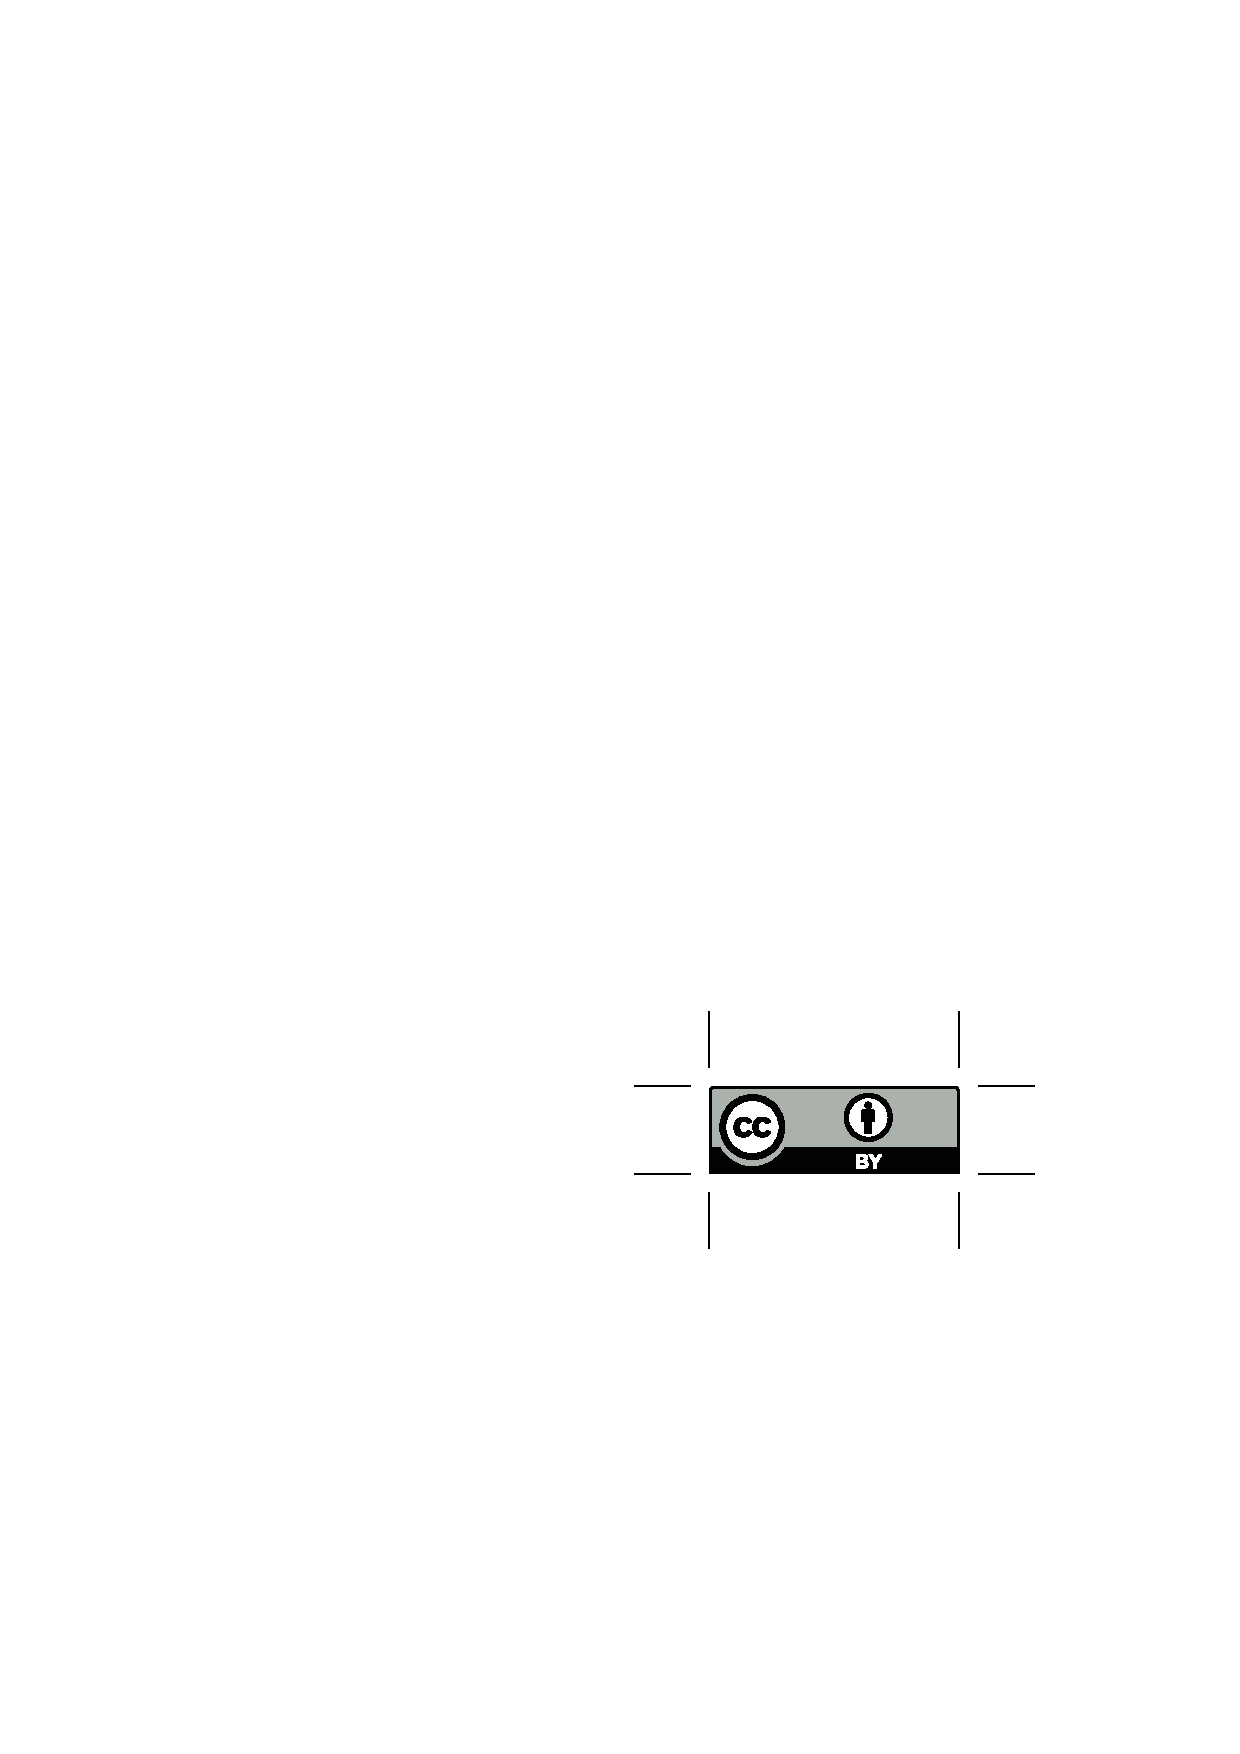
\includegraphics[width=0.90\textwidth]{by}}
  \end{minipage}\hfill
  \begin{minipage}{0.8\columnwidth}
   \href{https://creativecommons.org/licenses/by/4.0/}{This work is licensed under a Creative Commons Attribution International 4.0 License.}
  \end{minipage}
  \vspace{5pt}
}
\makeatother

\setcopyright{ifaamas}
\acmConference[AAMAS 2027]{Proc.\@ of the 26th International Conference
on Autonomous Agents and Multiagent Systems (AAMAS 2027)}{3--7 May 2027}{Hanoi, Vietnam}{M.~Baldoni, F.~Fang, W.~Yeoh, N.~Yorke-Smith (eds.)}
\copyrightyear{2027}
\acmYear{2027}
\acmDOI{}
\acmISBN{}

\acmSubmissionID{<<OpenReview submission id>>}
\submissionType{Research Paper Track}

%%% A loud marker for anything that awaits a real number. Delete the
%%% definition once the experiments are in and every use is gone.
\newcommand{\TODORESULT}[1]{\textbf{[TODO: #1]}}

\title{Does Agentic Collaboration Produce Scientific Innovation?}

\author{Anonymous Author(s)}
\affiliation{
  \institution{Anonymous Institution}
  \city{}
  \country{}}
\email{anonymous@example.com}

\begin{abstract}
Multi-agent systems of large language models are increasingly proposed as
engines of scientific discovery, and the case for using many agents rather
than one rests on an assumption that is rarely tested: that the agents build
on each other's work. We put that assumption on a substrate designed to let
it succeed or fail visibly. The published literature becomes a frozen,
read-only citation network of research ideas --- external background
knowledge that no agent can alter. Everything the agents write goes instead
to a \emph{shared board}: a separate network that every agent can search,
read and edit, and that starts empty. The only thing that evolves is the
board, so the board's trajectory is the object of study. Specialization is a
soft, continuous dial: each agent is told it is interested in $k$ topics drawn
from a pool of 128, and nothing in the environment enforces that interest ---
an agent may read anything and simply ignores what it does not want. Because
$k$ governs what an agent searches for in the literature and on the board
alike, it also governs how often two agents meet. We sweep $k$ from a single
topic to the whole pool and ask whether agents ever cite one another, whether
the board grows into a connected structure or a set of disconnected stars, and
whether ideas get better when they do. \TODORESULT{one sentence stating what
the $k$ sweep found} \TODORESULT{one sentence stating whether team size stops
being a pure throughput knob}
\end{abstract}

\keywords{Multi-agent systems; large language models; scientific discovery;
stigmergy; shared memory; emergent collaboration}

\begin{document}

\maketitle

\section{Introduction}

A system of language-model agents, given the recent scientific literature and
asked to propose new research, is now a familiar
construction~\cite{lu2024aiscientist,si2024llmideas}. The argument for making
it \emph{multi}-agent is an argument about collaboration: many agents explore
in parallel, encounter different corners of the literature, and --- the
assumption goes --- compound one another's partial results into something no
single agent would reach.

That last step is rarely measured. A prior study of LLM agents navigating a
16{,}208-node idea network found that team size behaved as a pure throughput
knob: per-idea quality was flat from 10 to 150 agents while the absolute
number of good ideas grew linearly, and across 10{,}300 actions exactly one
agent cited an idea that another agent had written.\footnote{Cited in third
person to preserve anonymity; see the anonymized supplement.} Parallelism, not
collaboration.

We think that result was, in part, an artifact of where the agents' output
went. In that system a generated idea was written into the \emph{same} graph
as the corpus, where it sat among sixteen thousand published papers,
indistinguishable from them and effectively invisible. An agent that wanted to
find a teammate's contribution had no way to ask for one.

This paper rebuilds the substrate so that the question can be answered rather
than assumed. We separate the two things that were conflated:

\begin{itemize}
\item The \textbf{literature} is a frozen citation network of research ideas
  distilled from published papers. It is external background knowledge. Agents
  search it, browse it and cite it, and no action can alter it --- read-only is
  a property of the object, enforced and tested, not a convention.
\item The \textbf{board} is a separate network holding everything the agents
  write. It starts empty. Every agent can search it, read it, post to it, and
  adjust the reference links on any post, including posts written by others.
\end{itemize}

Because the literature is fixed, the board is the only part of the state that
evolves. The dynamical system under study is therefore the board's trajectory:
how it grows, what shape it takes, and whether the posts on it ever point at
one another.

\paragraph{Specialization as a soft dial.}
An agent's disposition is set by a list of $k$ topics, drawn uniformly at
random from a pool of 128 derived from the corpus, and placed only in its
system prompt. The environment filters nothing: any agent may read any node in
either store, and material outside its interests simply gets skimmed and
dropped. This matters for the question at hand, because $k$ governs what an
agent goes looking for on the board as much as in the literature. At $k{=}1$
two agents rarely have anything to say to each other; at $k{=}128$ every agent
is interested in everything. \textbf{The probability that collaboration is even
possible is a function of $k$}, which is why we need no separate switch to turn
the channel on and off --- such a switch would duplicate the dial by a
mechanism independent of it.

\paragraph{Questions.}
\begin{enumerate}
\item Do agents cite each other at all, once contributions are addressable?
  Does the board become connected, or remain a set of isolated posts?
\item How does that depend on $k$ --- is there a breadth at which collaboration
  becomes likely?
\item Does collaboration, where it occurs, improve the ideas? We score each
  idea by whether a real paper published later realizes it.
\item Does team size stop being a pure throughput knob?
\end{enumerate}

\paragraph{Contributions.}
\begin{itemize}
\item An environment that separates immutable background knowledge from a
  shared, collectively editable workspace, with the read-only property enforced
  by construction and verified by an invariant test after every run.
\item A continuous specialization dial that is dispositional rather than
  enforced, and that couples an agent's reading to its chance of meeting a
  teammate.
\item \TODORESULT{the empirical finding, stated once the $k$ sweep is in}
\end{itemize}

\section{Related Work}

\paragraph{LLM agents for research ideation.}
Systems that generate and screen research ideas with language
models~\cite{lu2024aiscientist,si2024llmideas} are typically evaluated by human
preference or by rubric. We instead score against the arrow of time: an idea
counts only if a real paper published after the agent model's training cutoff
realizes it (\S\ref{sec:eval}).

\paragraph{Indirect coordination.}
Coordinating through a shared environment rather than through messages is
stigmergy~\cite{theraulaz1999stigmergy}; blackboard architectures are its
classical form in AI. Our board is a blackboard in that sense, with two
departures: it is the \emph{only} channel between agents, and it is
collectively editable, so an agent can revise the reference structure of
another's post.

\paragraph{Science of science.}
The structure of citation networks and the effect of team size and atypical
recombination on impact have been studied at scale on human
data~\cite{fortunato2018science,uzzi2013atypical,wu2019teams}; networks of this
kind grow by preferential attachment~\cite{barabasi1999emergence}. We ask which
of these regularities machine dynamics reproduce.

% TODO(refs): add blackboard architectures (Hayes-Roth 1985); recent
% multi-agent LLM frameworks; shared-memory / scratchpad agent work.

\section{The Environment}

\subsection{State: two stores}

The \textbf{corpus} is a directed graph whose nodes are one-paragraph idea
summaries of published papers and whose edges are citations. It is frozen after
loading: every mutating operation raises an error, and node payloads handed to
callers are detached copies, so no reference obtained through the API can be
used to alter it.

The \textbf{board} is a second directed graph, empty at the start of every run.
Node identifiers are disjoint by construction, so a single facade routes any
lookup to the right store. When a post cites a paper, the board holds a
text-free stub for that paper, which keeps every graph algorithm applicable to
the board without special cases and --- more importantly --- lets us separate
two structures that answer different questions: $\text{post} \to
\text{literature}$ edges say how deeply an idea is rooted in prior work, while
$\text{post} \to \text{post}$ edges are the direct evidence that agents
connected.

Each store has its own vector index. The corpus index is frozen with the
corpus; the board index grows as posts appear.

\subsection{Actions}

Navigation is symmetric across the two stores, which lets a single
implementation ablate either one independently:

\begin{table}[h]
\small
\begin{tabular}{@{}lll@{}}
\toprule
 & Literature & Board \\
\midrule
Semantic search & \texttt{search} & \texttt{search\_board} \\
Node and neighbors & \texttt{browse} & \texttt{browse\_board} \\
Random jump & \texttt{sample\_frontier} & \texttt{sample\_board} \\
\bottomrule
\end{tabular}
\end{table}

Three further actions write, and all of them target the board:
\texttt{generate} publishes a new idea citing whatever it builds on,
\texttt{add\_links} and \texttt{remove\_links} adjust the references of a post.
An agent chooses one action per turn by emitting a single JSON object, and
keeps a rolling memory of its last 20 (action, result) pairs.

\subsection{Write rules}

The source of any edge must be a board node; destinations may lie in either
store. Corpus-internal edges can therefore neither be added nor removed. There
is no ownership check: any agent may edit any post's links, which makes
``adding a citation to a teammate's post'' an available and observable act of
uptake.

\subsection{Specialization}

Each agent draws $k$ distinct topics uniformly at random from a pool of 128
obtained by clustering the corpus embeddings and naming each cluster. The draws
are seeded and recorded. Topics appear only in the agent's system prompt;
nothing in the environment enforces them. With $N$ agents drawing from 128
topics, overlap is unavoidable above a certain $N$ and grows with $k$ --- that
overlap is the substrate collaboration needs, and we report it as a mediating
variable rather than treating it as a constant.

\section{Evaluation}
\label{sec:eval}

\paragraph{Headline: anticipation.}
For each generated idea we extract three literature-search queries, retrieve
candidates from two scholarly APIs~\cite{kinney2023s2,priem2022openalex}, and
have an LLM judge grade each candidate on a six-point realization scale across
three cumulative venue-recognition tiers. Candidates published on or before the
agent model's training cutoff, and candidates that are corpus members, are
excluded before scoring. The headline metric is the share of ideas whose best
match reaches ``same specific problem'' or better. Because probe tests show the
model's parametric memory extends months past its official cutoff, only
realizations published at least eight months after that cutoff count.

\paragraph{Mechanism: the board's structure over time.}
Every structural quantity is a function of round, computed by replaying the
event log: the share of $\text{post}\to\text{post}$ edges among all board
edges, the number of connected components, the step of the first citation of
another agent's post, the depth of the longest citation chain, and the
in-degree distribution over posts.

\paragraph{A new observable.}
Because the environment filters nothing, the event log records what an agent
retrieved but did not use. A non-citation is therefore no longer ambiguous
between \emph{never surfaced} and \emph{surfaced and declined} --- a
distinction the earlier system could not draw, and one that separates ``the
channel is closed'' from ``the channel is open and unused''.

\section{Experiments}

\subsection{Setup}

The corpus holds 16{,}208 ideas distilled from papers published 2020--2024 at
four machine-learning venues. Agents are driven by a single frontier
language model; the judge, the summarizer and the topic namer are a smaller
model from the same family. Each run is 80 rounds --- every agent acts once per
round --- under one seed.

\subsection{The specialization sweep}

$k \in \{1, 2, 4, 8, 16, 32, 64, 128\}$ at $N{=}10$, eight runs. $k{=}128$ is
the whole pool: every agent interested in everything, the generalist endpoint.

\TODORESULT{Table: per-$k$ anticipation accuracy, ideas produced, share of
post$\to$post edges, components, first cross-agent citation step}

\TODORESULT{Figure: board structure as a function of round, one line per $k$}

\subsection{Team size}

The shape of the team-size sweep is deliberately deferred until the $k$ sweep
is read: $N$ must be swept at more than one $k$ for any bend in the curve to be
attributable to collaboration rather than to that particular breadth.

\TODORESULT{$N$ sweep design and results}

\subsection{Navigation ablations}

Because navigation is symmetric, search, link-following and random jumps can be
disabled on the literature and on the board independently.

\TODORESULT{ablation results}

\section{Limitations}

\paragraph{The dial spans machine learning, not computer science.}
The 128 topics are clusters of a corpus drawn from four machine-learning
venues. They cover that field densely and contain essentially nothing from
databases, networking, operating systems, architecture, programming languages,
cryptography, human-computer interaction or visualization. ``Specialist'' and
``generalist'' here mean narrow and broad \emph{within machine learning}. Note
the deliberate asymmetry with evaluation, which recognizes realizations at
venues across computer science: an idea realized outside machine learning
counts, even though no agent could have read that literature.

\paragraph{Single seed.}
\TODORESULT{state the replicate evidence and the noise band once runs exist}

\paragraph{One agent model, one judge.}
The dynamics are those of a single model, and the judge is a smaller model
whose rubric we audit but do not calibrate against human experts at scale.

\paragraph{Collaboration is not messaging.}
The board is the only channel. Agents cannot address one another, negotiate, or
divide labour explicitly. A negative result here bounds \emph{stigmergic}
collaboration, not collaboration in general.

\section{Conclusion}

\TODORESULT{the conclusion, once the $k$ sweep is in. If post$\to$post edges
appear, the story is how collaboration emerges with breadth; if they do not,
the story is that the channel was open and went unused, which is a different
and sharper claim than the earlier system could support.}

\balance
\bibliographystyle{ACM-Reference-Format}
\bibliography{references}

\end{document}
